\documentclass[letterpaper,10pt]{article}

\usepackage{csquotes}
\usepackage{titling}
\usepackage{listings}
\usepackage{url}
\usepackage{setspace}
\usepackage{subfig}
\usepackage{sectsty}
\usepackage{pdfpages}
\usepackage{colortbl}
\usepackage{multirow}
\usepackage{multicol}
\usepackage{relsize}
\usepackage{amsmath}
\usepackage{wasysym}
\usepackage{fancyvrb}
\usepackage{amsmath,amssymb,amsthm,graphicx,xspace}
\usepackage[titlenotnumbered,noend,noline]{algorithm2e}
\usepackage[compact]{titlesec}
\usepackage{XCharter}
\usepackage[T1]{fontenc}
\usepackage{tikz}
\usetikzlibrary{arrows,automata,shapes,trees,matrix,chains,scopes,positioning,calc}
\tikzstyle{block} = [rectangle, draw, fill=blue!20, 
    text width=2.5em, text centered, rounded corners, minimum height=2em]
\tikzstyle{bw} = [rectangle, draw, fill=blue!20, 
    text width=4em, text centered, rounded corners, minimum height=2em]

\definecolor{namerow}{cmyk}{.40,.40,.40,.40}
\definecolor{namecol}{cmyk}{.40,.40,.40,.40}

\let\LaTeXtitle\title
\renewcommand{\title}[1]{\LaTeXtitle{\textsf{#1}}}


\newcommand{\handout}[5]{
  \noindent
  \begin{center}
  \framebox{
    \vbox{
      \hbox to 5.78in { {\bf ECE459: Programming for Performance } \hfill #2 }
      \vspace{4mm}
      \hbox to 5.78in { {\Large \hfill #4  \hfill} }
      \vspace{2mm}
      \hbox to 5.78in { {\em #3 \hfill} }
    }
  }
  \end{center}
  \vspace*{4mm}
}

\newcommand{\lecture}[3]{\handout{#1}{#2}{#3}{Lecture #1}}
\newcommand{\tuple}[1]{\ensuremath{\left\langle #1 \right\rangle}\xspace}

\addtolength{\oddsidemargin}{-1.000in}
\addtolength{\evensidemargin}{-0.500in}
\addtolength{\textwidth}{2.0in}
\addtolength{\topmargin}{-1.000in}
\addtolength{\textheight}{1.75in}
\addtolength{\parskip}{\baselineskip}
\setlength{\parindent}{0in}
\renewcommand{\baselinestretch}{1.5}

\singlespace

\title{\bf ECE 459: Programming for Performance\\Assignment 2}
\author{Patrick Lam \& Jeff Zarnett\\
\small{With acknowledgement and thanks to Douglas Harder and Stephen Li}}
\date{\today ~ (Due: February 12, 2020)}

\lstset{basicstyle=\scriptsize, frame=single}

\begin{document}

\maketitle
% http://gurmeet.net/2008/09/20/latex-tips-n-tricks-for-conference-papers/
\newcommand{\squishlist}{
 \begin{list}{$\bullet$}
  { \setlength{\itemsep}{0pt}
     \setlength{\parsep}{3pt}
     \setlength{\topsep}{3pt}
     \setlength{\partopsep}{0pt}
     \setlength{\leftmargin}{1.5em}
     \setlength{\labelwidth}{1em}
     \setlength{\labelsep}{0.5em} } }
\newcommand{\squishend}{
  \end{list}  }

\noindent
Important Notes:

\squishlist
  \item Make sure you run your program on {\tt ecetesla0.uwaterloo.ca}.
  \item Use the command ``{\tt OMP\_NUM\_THREADS=14;export OMP\_NUM\_THREADS}'' to set 14 threads.
\squishend

\paragraph{Using \texttt{hyperfine}.} 
A student suggested \texttt{hyperfine} as a benchmarking tool and it's a good
idea. This allows you to collect data for multiple
runs of your program easily and reliably! I recommend that you take a moment
to look at the documentation at \url{https://github.com/sharkdp/hyperfine}. 
The default options are mostly fine, but add \texttt{-}\texttt{-warmup 1}. 
Make sure you put the full command to run in single quotes. It does hide the
standard output, so make sure your program is correct before benchmarking.
See the example below.

\begin{center}
	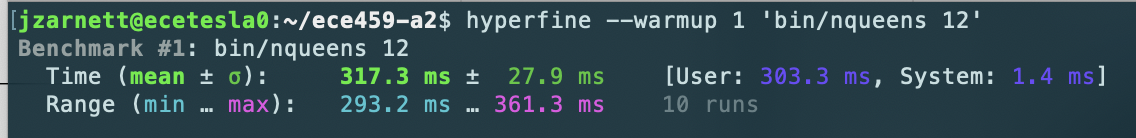
\includegraphics[width=\textwidth]{images/hyperfine.png}
\end{center}

You want to report all these values in your report. If you get warnings about
statistical outliers, you should re-run your benchmark. However, if you are
doing the test at a time when the system is very busy, you will always get 
this result. If you are unable to try again later when the system is less
busy, then just be sure to explain in your report that you got this warning.
TAs will probably test when things are less busy, so their results may vary.


\section{Automatic Parallelization (15 marks)}
Ray tracing is, in principle, easy to automatically parallelize. You do
a separate computation for each point. In this part, you will convince a
parallelizing compiler (Oracle's Solaris Studio) to parallelize
a simple raytracing computation.

For this question, you will work with {\tt raytrace\_simple.c} and {\tt
  raytrace\_auto.c} in the {\tt q1} directory.  I've bumped up the
height of the image to 60000 pixels so that the compiler will find it
profitable to parallelize. Benchmark the sequential ({\tt raytrace})
and optimized sequential ({\tt raytrace\_opt}) versions. Note that the
compiler does manage to significantly optimize the computation of the sequential
raytrace. Report the speedup due to the compiler and
speculate why that is the case. Compare all subsequent numbers
to the optimized version.

Your first programming task is to modify your program so you can take
advantage of automatic parallelization. Determine what why it won't
parallelize as is, and make any changes necessary. Preserve behaviour
and make all your changes to {\tt raytrace\_auto.c}.

Solaris Studio 12.3 is available on {\tt ecetesla0}. The provided {\tt
  Makefile} calls that compiler with the relevant flags. Your compiler
output should look something like the following (the line numbers
don't have to match, but you {\bf must} parallelize the critical loop):

\begin{lstlisting}
Compiling Part 1 Automatic Parallelization
/opt/oracle/solarisstudio12.3/bin/cc  -fast -xautopar -xloopinfo -xreduction -xbuiltin -xO4 \
    src/raytrace_auto.c -o bin/raytrace_auto
"raytrace_auto.c", line 217: PARALLELIZED
"raytrace_auto.c", line 218: not parallelized, not profitable
"raytrace_auto.c", line 233: not parallelized, loop has multiple exits
"raytrace_auto.c", line 241: not parallelized, not a recognized for loop
"raytrace_auto.c", line 264: not parallelized, not a recognized for loop
\end{lstlisting}

Justify each change you make and explain why:
\begin{itemize}
\item the existing code does not parallelize;
\item your changes improve parallelization and preserve the behaviour of the sequential version
\item your changes adversely impact maintainability
\end{itemize}

Run your benchmark again and calculate your speedup. Speculate about why you got your speedup. Speedup is calculated using \texttt{hyperfine}.

\squishlist
  \item {\bf Minimum expected speedup:} 10x over \texttt{bin/raytrace}, 5x over \texttt{bin/raytrace\_opt}
  \item {\bf (my) initial solution speedup (real time):} 12.6x over \texttt{bin/raytrace}, 7.6x over \texttt{bin/raytrace\_opt}
\squishend

\paragraph{Totally unrelated hints.} Consider this page:
\begin{center}
  \scriptsize \url{http://stackoverflow.com/questions/321143/good-programming-practices-for-macro-definitions-define-in-c}
\end{center}
Also, let's say that you want a macro to return a struct of type {\tt struct foo} with
two fields. You can create such a struct on-the-fly like so: \verb!(struct foo){1,2}!.

\section{Using OpenMP Tasks (30 marks)}

We saw briefly how OpenMP tasks allow us to easily express some parallelism.
In this question, you will apply OpenMP tasks to the $n$-queens
problem\footnote{\url{https://en.wikipedia.org/wiki/Eight\_queens\_puzzle}}.
Benchmark the provided sequential version with a number that executes in approximately
15 seconds under {\tt -O2} (14 on {\tt ecetesla0} takes roughly 13.4s, but 15 takes about 1m 25s. 
So choose 14 in this scenario.).

\noindent {\bf Notes:} Use {\tt er\_src} to get more detail about what the Oracle
Solaris Studio compiler did.  You may change the
Makefile's compilation flags if needed. Report speedups over the
compiler-optimized sequential version.  You can use any compiler, but
say which one you used. OpenMP tips:
  \url{www.viva64.com/en/a/0054/}

Modify the code to use OpenMP tasks. Benchmark your modified program
and calculate the speedup. Explain why your
changes improved performance. Write a couple of sentences explaining how
you could further improve performance.

\vspace*{1em}
\noindent {\bf Hints:} 1) Be sure to get the right variable scoping, or
you'll get race conditions. 2) Just adding the task annotation is going
to make your code way slower. 3) You will have to implement a cutoff to
get speedup. See, for instance, the Google results for ``openmp
fibonacci tasks''. 4) My solution includes 4 annotations and some
cutting-and-pasting of code. 5) Be sure to check the output of the
OpenMP program for a given input against the non-OpenMP program to be
sure that your results are consistent.

\squishlist
  \item {\bf Minimum expected speedup:} 4x with n=13, 1.75x with n=14 
  \item {\bf Initial solution speedup:} 5x with n=13, 2x with n=14
\squishend


\section{Manual Parallelization with OpenMP (55 marks)}

This time rather than just apply OpenMP directives to an existing program, you will write the program according to what is written below and verify its correctness with some provided sample inputs.

Many web applications use JSON Web Token (JWT) for user authentication. A JWT is composed of three components: a header, a payload, and a signature. All three components are encoded using the Base64URL algorithm and concatenated together with dots. The header and payload components are JSON objects specific for each application but can mostly be ignored for the purpose of this assignment. The signature component that authenticates the information in the header and payload is generated using HMAC-SHA256 algorithm as shown below.

\begin{verbatim}
HMACSHA256(
  base64UrlEncode(header) + "." +
  base64UrlEncode(payload),
  secret)
\end{verbatim}

The \textquote{secret} is what prevents malicious actors from generating fake JWT. Your task is to write a program that brute forces a JWT's secret. Your program will be given three inputs on the command line: (1) the JWT, (2) maximum length of the secret, and (3) an alphabet representing the set of possible characters in the JWT's secret. For example, the alphabet \textquote{abcdefghijklmnopqrstuvwxyz0123456789} represents the set of lowercase letters and numeric digits. Once you found the secret, your program should print it out in \texttt{stdout}.

Note that in practice, a JWT secret should be 32 bytes long, making it impractical to brute force. For the purpose of this assignment, we will be using small secrets that can be brute forced within a reasonable timeframe. Please don't try to use this code on UW hardware to crack anything other than some test data for this exercise. The test data is sufficiently small that you can crack it in a few minutes; if it's taking much longer than that, something is wrong.

Once the sequential version is written, you will apply OpenMP directive(s). It's recommended to add them one at a time, or a related group at a time, to see what works and what doesn't. 

To produce the data we want for the report, the easiest way is just to take notes about what about OpenMP directives you have used. Each time you add some OpenMP directive(s), note down what it was and what effect it had, if any. By writing down what was successful and what was not, as well as what made a big difference, you will have at hand all the data you need.

You should also try to achieve the maximum speedup you can while preserving behaviour. The usage of the compiled output is: \texttt{./jwtcracker jwt maxsecretlen alphabet}. This behaviour needs to be preserved for your solution to be tested.

Submit the final OpenMP-annotated version of your code. Your report will contain the impact of various OpenMP directives, walking the reader through the process of applying them and testing out their effectiveness.

\squishlist
  \item {\bf Minimum expected speedup:} 2
  \item {\bf Initial solution speedup:} 2.4
\squishend

\newpage
\section*{Rubric}

The general principle is that correct solutions earn full marks.
However, it is your responsibility to demonstrate to the TA
that your solution is correct. Well-designed, clean solutions 
are therefore more likely to be recognized as correct. 

Solutions that do not compile will earn at most 39\% of the available
marks for that part. Segfaulting or otherwise crashing solutions earn
at most 49\%.

\paragraph{Part 1, Automatic Parallelization (15 marks):}  
\begin{itemize}
\item 10 marks for implementation: A correct solution must:
\begin{itemize}
	\item preserve the behaviour (5 points); and
	\item enable additional parallelization (5 points).
\end{itemize}
 
\item 5 marks for report: include the necessary information
(describing the experiments and results, reasonably speculating about
the cause, and explaining why you preserve behaviour)
\end{itemize}

\paragraph{Part 2, OpenMP Tasks (30 marks):} 

\begin{itemize}
\item 20 marks for implementation: A correct solution must:
\begin{itemize}
	\item properly use OpenMP tasks to get a speedup;
	\item be free of obvious race conditions.
\end{itemize}
\item 10 marks for report: 
\begin{itemize}
\item 7 marks for analyzing the performance
of the provided version, describing the speedup due to your
changes, explaining why your changes improved performance, and
speculating reasonably about further changes. 
\item 3 marks for clarity.
\end{itemize}
\end{itemize}

\paragraph{Part 3, Manual Parallelization (55 marks):} 
\begin{itemize}
\item 35 marks for the single-threaded implementation. 

\item 10 marks for the use of OpenMP pragmas and minor code changes to parallelize the code and get speedup.

\item 10 marks for report: Explain which OpenMP directives helped and why. 3 marks for clarity.
\end{itemize}



\end{document}

